\section{Other Systematic uncertainties}
\label{Systematic uncertainty}
Before we proceed this section, we state some systematic uncertainties mentioned in previous sections, and add some conclusions on those which are simple to handle as follow,
\begin{itemize}
    \item re-weight of \pt distribution from high- and low-multiplicity samples (for ratios of \effAcc and the other efficiencies),
    \item re-weight of $y^*$ distribution from high- and low-multiplicity samples (for ratios of \effAcc and the other efficiencies),
    \item uncertainties due to the limit calibration sample size in PIDCalib efficiency table (for ratios of efficiencies except \effAcc),
    \item uncertainties of data-over-simulation ratio of per tracking efficiency(for ratios of efficiencies except \effAcc),
    \item global cut of nVeloClusters $<8000$ (negligible),
    \item uncertainty of luminosity is canceled when calculating the ratio of \psitwos-to-\jpsi production,
    \item relative uncertainty due to branching fraction is calculated to be $2.2\%$, this term is not considered when calculating the normalized ratio as function of multiplicity, but when we compare ratio in forward and backward regions, we do not normalize the ratio, hence, need to consider it in this case.
\end{itemize}

Other systematic uncertainties are reported in this section.
\subsection{Monte Carlo statistics}
This uncertainty is the statistical error on the ratio of efficiencies in different multiplicity bins, due to the finite size of the simulation samples. The uncertainty varies from $0.02\%$ to $0.2\%$ over all multiplicity classes divided by three multiplicity variables and in $p$Pb and Pb$p$ configurations, which is negligible compared to other systematic uncertainties.
\subsection{Signal extraction}
The choice of the fit model for the mass and $t_z$ distributions affects the number of events. In Sec~\ref{Signal extraction} we have mentioned that two CB functions with common mean are used for \jpsi mass fit while only one is used for \psitwos. The uncertainty associated with the choice of the signal mass function is estimated using a different function of two CB functions for \psitwos. Two CB functions have common mean, the $\alpha$ values for both CB functions are determined by the Eq.~\ref{alphasigma}. And the width of wider CB function is determined by $\sigma_2=sigma_1+25.7$, the ratio of the narrower one is fixed to 0.96 according to the study in 13.TeV $pp$ collisions~\cite{LHCb:2019eaj}.
New fit model for \psitwos mass spectrum is introduced and then a new two-dimensional fit for mass and $t_z$ is performed. Then the difference in ratio of \psitwos-to-\jpsi ratio and the statistical uncertainty of the ratio in each $N_{\rm tracks}^{\rm PV}$ bin are shown in Figure~\ref{StatsAndFit}.
\begin{figure}[H]
\begin{center}
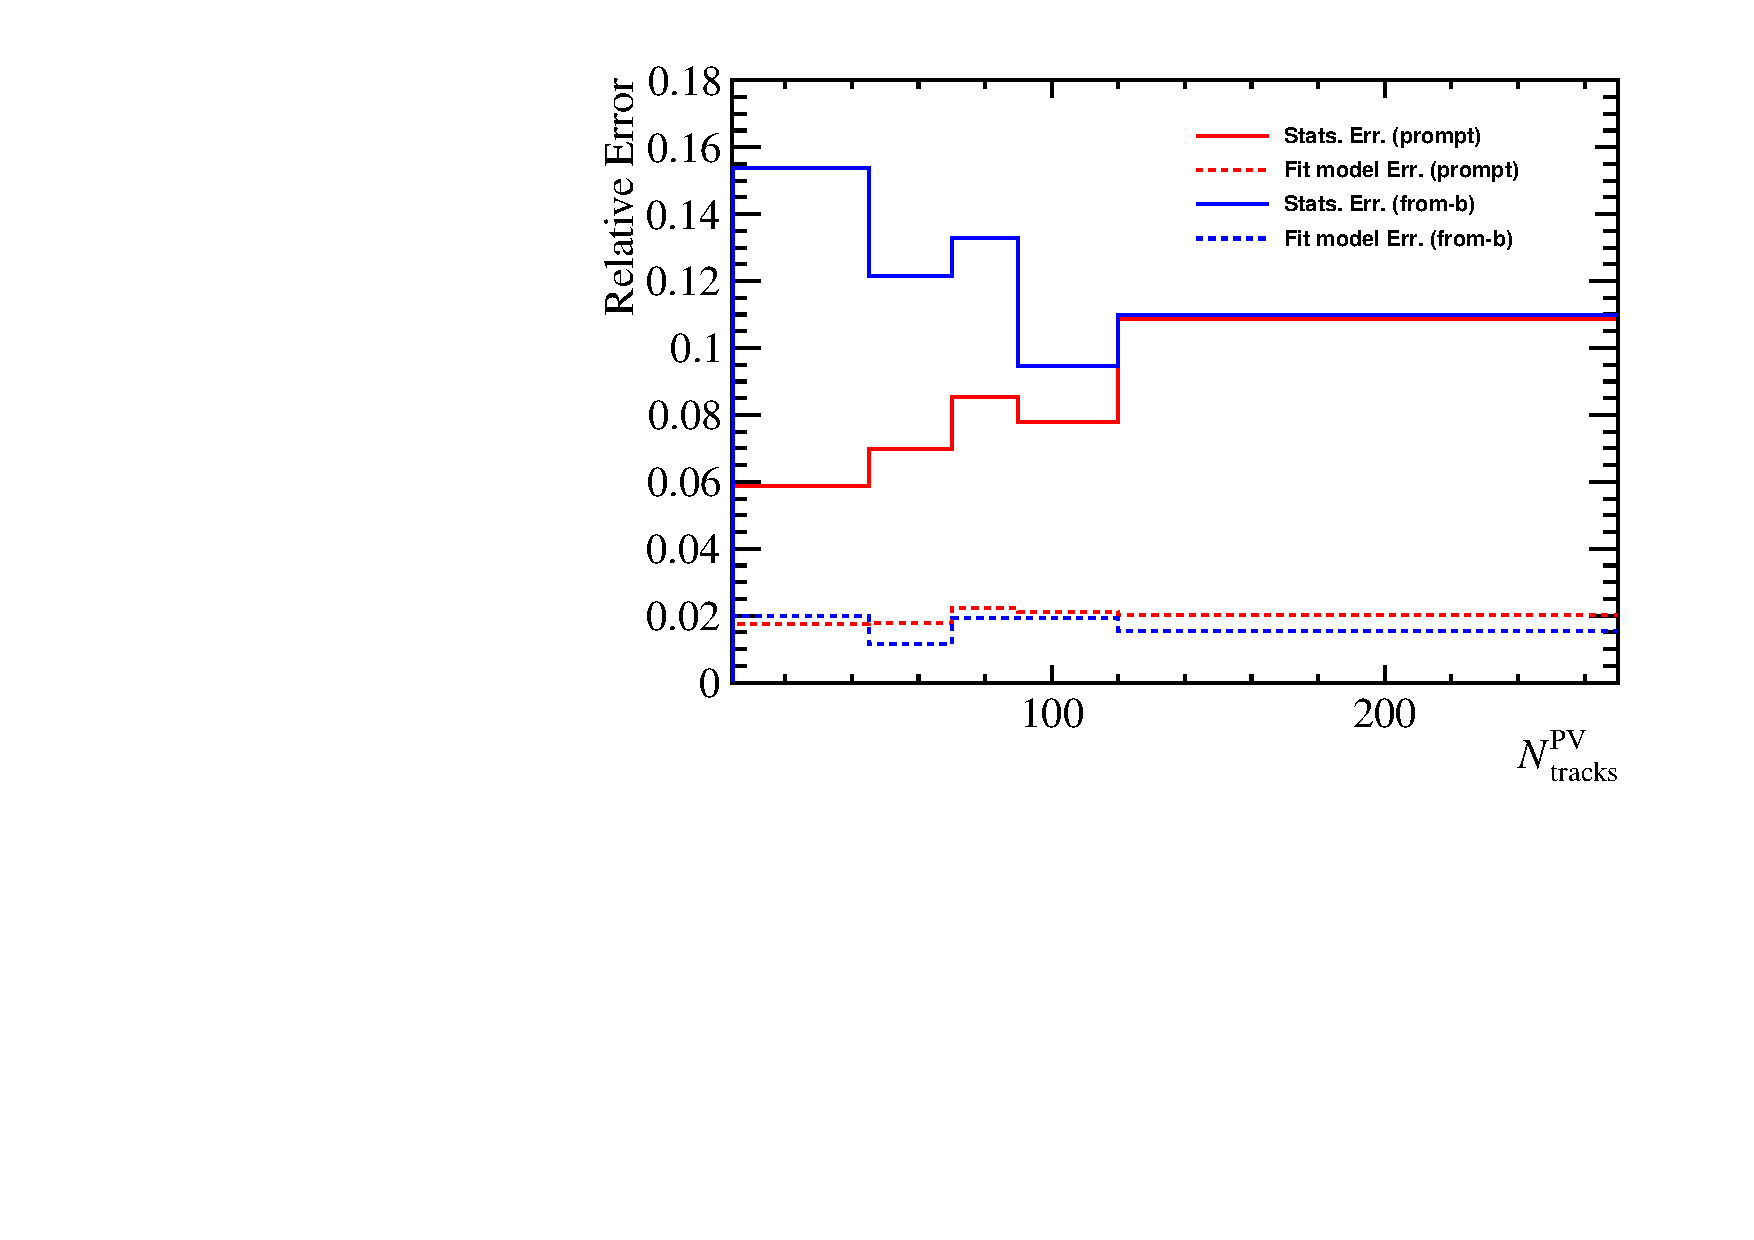
\includegraphics[width=0.7\linewidth]{pdf/pPb/Workdir/SysErr/FitModel.pdf}
\end{center}
\caption{
        The statistical uncertainties and the systematic uncertainty arised from different fit model of \psitwos-to-\jpsi ratio.}
\label{StatsAndFit}
\end{figure}
We can see that the variation caused by different fit model is totally merged by the statistical uncertainties, the statistical uncertainty is larger than the uncertainty caused by fit model by at least a factor of 3. Which means we can completely treat the difference caused by fit model as statistical fluctuation, hence, negligible.

\subsection{Trigger efficiency}
The trigger efficiency in simulation is cross-checked with data, and the resulting difference in the ratio of \effTrigger between simulation and data is quoted as a systematic uncertainty. If the statistical uncertainties of the ratio arised from fitting the TIS and TISTOS sample of \jpsi and \psitwos are larger, then it will be quoted as systematic uncertainty. 
For both L0Muon and Hlt1DiMuonHighMass the TISTOS method is used to evaluate the efficiency for L0Muon \&\& Hlt1DiMuonHighMass both in simulation and data. We use L0Global as the TIS line. As the data sample size is limited by the number of the TIS events of \psitwos sample, the TISTOS efficiencies derived by data and Monte Carlo sample over all multiplicity and kinematic region. Due to the different global cuts under different multiplicity schemes and configurations, TISTOS method is carried out in each case and the result is summarized in Table~\ref{TISTOStable}.
\begin{table}[H]
\caption{Systematic uncertainty of \effTrigger by TISTOS method.}
\begin{center}
\begin{tabular}{lllll}
\hline
\textbf{Configuration} & \textbf{Mult. Variable} & \textbf{Variation} & \textbf{Stats. Err.} & \textbf{Syst. Err. quoted}  \\
\hline
	$p$Pb & $N_{\rm tracks}^{\rm PV}$ & 2.7\% & 3.9\% & 3.9\%\\
	$p$Pb & $N_{\rm fwd}^{\rm PV}$ & 3.2\% & 3.0\% & 3.2\%\\
	$p$Pb & $N_{\rm bwd}^{\rm PV}$ & 2.7\% & 3.9\% & 3.9\% \\
        Pb$p$ & $N_{\rm tracks}^{\rm PV}$ & 2.0\% & 3.8\% & 3.8\% \\
        Pb$p$ & $N_{\rm fwd}^{\rm PV}$ &  1.7\% & 3.6\% & 3.6\%\\
        Pb$p$ & $N_{\rm bwd}^{\rm PV}$ &  2.7\% & 4.1\% & 4.1\%\\
\hline
\end{tabular}
\label{TISTOStable}
\end{center}
\end{table}
\subsection{Binning scheme of PID table}
Uncertainty due to binning scheme of the calibration sample, studied by varying the binning method in $p_\mu$, $\eta_\mu$, and nSPDHits respectively. The default one and the two alternative binning schemes could be found below. The nominal binning scheme of the muon ID efficiency for muons we use to calculate the muon ID efficiency of \jpsi and \psitwos mesons is defined:
\begin{itemize}
  \item $p_\mu$ boundaries [\gevc]: 3, 10, 20, 25, 30, 35, 40, 45, 50, 60, 70, 80, 100, 1000.
  \item $\eta$ boundaries: 2.0, 2.5, 3.0, 3.5, 4.0, 4.5, 5.0.
  \item nSPDhits boundaries: 0, 300, 500, 700, 1400.
\end{itemize}

One of the two alternative binning schemes is defined:
\begin{itemize}
  \item $p_\mu$ boundaries [\gevc]: 3, 12.5, 22.5, 27.5, 32.5, 37.5, 42.5, 47.5, 55, 65, 75, 85, 100, 1000.
  \item $\eta$ boundaries: 2.0, 2.6, 2.9, 3.6, 3.9, 4.5, 5.0.
  \item nSPDhits boundaries: 0, 250, 450, 650, 1400.
\end{itemize}

The other one binning schemes is defined:
\begin{itemize}
  \item $p_\mu$ boundaries [\gevc]: 3, 9, 19, 24, 29, 34, 39, 44, 49, 59, 69, 79, 100, 1000.
  \item $\eta$ boundaries: 2.0, 2.4, 3.1, 3.4, 3.9, 4.5, 5.0.
  \item nSPDhits boundaries: 0, 320, 480, 720, 1400.
\end{itemize}
The maximum difference between the two new ratios calculated and the nominal ratio is quoted as the systematic uncertainty. The uncertainties are from 0.1\% to 1.8\%.

\subsection{Summary of systematic uncertainties}
All the systematic uncertainties are summarized in Table~\ref{AllSysErr}.
\begin{table}[H]
\caption{Summary of systematic uncertainties on \psitwos-to-\jpsi cross-section ratio.}
\begin{center}
\begin{tabular}{llll}
\hline
\textbf{source} & \textbf{$p$Pb} & \textbf{Pb$p$} \\
\hline
L0\&HLT & 3.2\%-3.9\% & 3.6\%-4.1\% \\
\hline
	Tracking Table Uncertainty\& & & \\
	PID Table Uncertainty\& & & \\
	\pt spectrum\& & & \\
	$y$ spectrum & 1.7\%-3.6\% & 2.1\%-3.6\% \\
\hline
	PID Table scheme & 0.4\%-1.7\% & 0.1\%-1.8\% \\
\hline
	Imperfectly simulating acceptance & 0.8\%-1.2\% & 0.9\%-1.3\% \\
\hline
	$\frac{\BR(\jpsi\rightarrow\mu^+\mu^-)}{\BR(\psitwos\rightarrow\mu^+\mu^-}$(canceled if normalized) & 2.2\% &2.2\% \\
\hline
	Fit model & negligible & negligible \\
\hline
	MC sample size & negligible & negligible \\
\hline
	Multiplicity global cut & negligible & negligible \\
\hline
\end{tabular}
\label{AllSysErr}
\end{center}
\end{table}

